\renewcommand{\NomeBloco}{\emph{Porta de Transmissão}}
\renewcommand{\NomeBlocoNoIt}{Porta de Transmissão}
\renewcommand{\NomePTab}{tab_\NomeBlocoNoIt}
\renewcommand{\NomeSTab}{tab_\NomeBlocoNoIt2}
\renewcommand{\NomePFig}{fig_\NomeBlocoNoIt}
\renewcommand{\NomeSFig}{fig_\NomeBlocoNoIt2}
\renewcommand{\NomeTTab}{tab_\NomeBlocoNoIt3}

\section{Porta de Transmissão}

O bloco \emph{\NomeBloco{}} funciona como uma chave, permitindo ou não o sinal de um lado passar ao outro. O bloco apresenta as defini ções de sinais de entrada e sa\'ida referidos na \autoref{\NomeSTab}.

\begin{table}[htbp]
\caption{Sinais do bloco \emph{\NomeBloco}}
\label{\NomeSTab}
\centering
\begin{tabular}{ccl}

    \toprule
    Sinal & Tipo    & Descri ção        \\
    \midrule \midrule
    A & Bidirecional & Sinal bidirecional 1\\
    \midrule
    B & Bidirecional & Sinal bidirecional 2\\
    \midrule
    ENABLE & Entrada & Sinal de habilita ção\\
    \bottomrule
\end{tabular}
\legend{Fonte: Produzido pelo autor}
\end{table}

O circuito projetado para o bloco \'e demonstrado na \autoref{\NomePFig}.

\begin{figure}[htb]
 \label{\NomePFig}
 \centering
  \begin{minipage}{0.4\textwidth}
    \centering
    \caption{Circuito CMOS projetado para o bloco \emph{\NomeBloco}} \label{\NomePFig}
    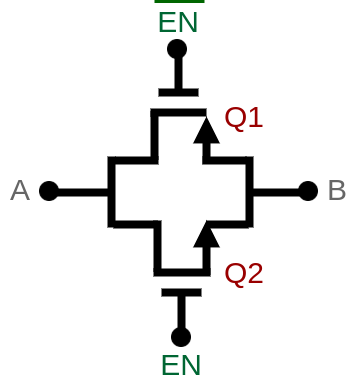
\includegraphics[scale=0.3]{Circuitos/TG.png}
    \legend{Fonte: Produzido pelo autor}
  \end{minipage}
  \hfill
  \begin{minipage}{0.4\textwidth}
    \centering
    \caption{Representa ção em bloco do \emph{\NomeBloco}} \label{\NomeSFig}
    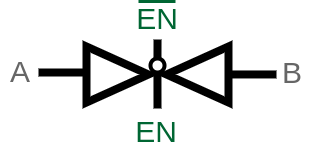
\includegraphics[scale=0.3]{Circuitos/TG_Simbolo.png}
    \legend{Fonte: Produzido pelo autor}
  \end{minipage}
\end{figure}

Os transistores utilizados no bloco \emph{\NomeBloco{}} apresentam os par\^ametros mostrados na \autoref{\NomeTTab}.

\begin{table}[htbp]
\caption{Transistores do Bloco \emph{\NomeBloco}}
\label{\NomeTTab}
\centering
\begin{tabular}{ccccc}
\toprule
Transistor & W ($\mu$m)  & L ($\mu$m)           & M (n° dispositivos) & S (n° dispositivos)\\
\midrule \midrule
Q1 & 0,8 & 0,18 & 1 & 1\\
\midrule
Q2 & 0,4 & 0,18 & 1 & 1\\
\bottomrule
\end{tabular}
\legend{Fonte: Produzido pelo autor}
\end{table}